% paper/sections/06_results.tex
% Results Section

Our $2\times2$ experiments cross the Suppression Filter (ON/OFF) with dyadic trust (ON/OFF). Each cell has $30$ runs of $200$ steps with seed $42+i$ for run $i$. Primary pairwise inference uses seed-paired Wilcoxon signed-rank tests. The lead scientific contrast is Baseline vs.\ Filter Only on retention (churn) and active $\sigma$; revenue is a scaled retention readout under fixed $M_{\mathrm{unsafe}}$. Adjusted $p$-values reported below come from a conservative Bonferroni secondary screen ($m=62$ non-degenerate pairwise contrasts; flat Trust-OFF trust KPIs excluded). Mann--Whitney $U$ is supplementary only. Cohen's $d=(\bar x_1-\bar x_2)/\mathrm{SD}_{\mathrm{pooled}}$ follows the printed Group1 vs.\ Group2 order (negative $d$ when Group2 is larger). For near-separated churn and revenue we emphasize mean differences and CIs; very large $|d|$ is a separation signal. SciPy's Wilcoxon $W$ is the minimum of the two signed-rank sums ($W=0$ indicates complete same-direction separation among nonzero paired differences). Primary polarization $\sigma$ is over \emph{active} agents; $\sigma_{\mathrm{all}}$ retains last opinions of churned agents. CSV condition labels retain the legacy name ``Bridge Only'' for Filter Only.

\subsection{The Polarization Paradox: Retention vs.\ Active-User Dispersion}
We begin with \textbf{Baseline} vs.\ \textbf{Filter Only}, isolating the Suppression Filter when trust is off. The tension between short-term retention and active-user polarization is the \textbf{Polarization Paradox}.

\subsubsection{User Retention and Platform Revenue}

In the unmoderated \textbf{Baseline}, cumulative churn reaches $39.18\%$ ($\text{SD} = 2.27\%$, $95\%\ \text{CI} = [38.39\%, 39.98\%]$) by step $200$, leaving $304.1$ active users on average ($\text{SD} = 11.35$, $95\%\ \text{CI} = [300.10, 308.03]$). Frustration among survivors is $0.9668$ ($\text{SD} = 0.1669$, $95\%\ \text{CI} = [0.9055, 1.0239]$). Final step-wise revenue averages \$121.64 ($\text{SD} = \$4.54$, $95\%\ \text{CI} = [\$120.04, \$123.21]$) under the constant unsafe multiplier---a readability scale on retention, not an independent brand-safety mechanism in this design.

Activating the Suppression Filter (\textbf{Filter Only}) cuts churn to $0.38\%$ ($\text{SD} = 0.30\%$, $95\%\ \text{CI} = [0.27\%, 0.49\%]$; mean difference $\approx -38.8$ percentage points; Figure~\ref{fig:churn}). Seed-paired Wilcoxon $W = 0.0$, $p_{\text{adjusted}} < 1.1 \times 10^{-4}$ (near-complete separation). Active users rise to $498.1$ ($\text{SD} = 1.52$, $95\%\ \text{CI} = [497.57, 498.63]$).

\begin{figure}[htbp]
    \centering
    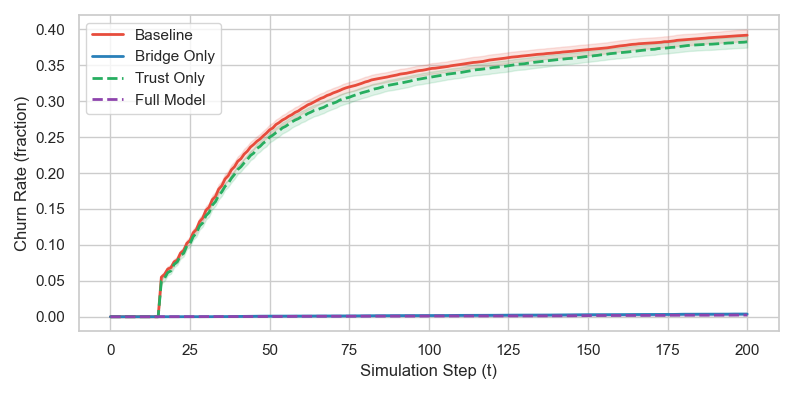
\includegraphics[width=0.58\textwidth]{figures/fig3_churn_factorial.png}
    \caption{Cumulative user churn rate over time ($N=500$, $30$ runs per condition). Filter Only mean final churn is $0.38\%$; Full Model is $0.21\%$; Filter OFF conditions show high attrition ($\approx 39\%$). Error ribbons: $95\%$ CIs.}
    \label{fig:churn}
\end{figure}

Mean frustration among active users falls to $0.5819$ ($\text{SD} = 0.0576$, $95\%\ \text{CI} = [0.5617, 0.6024]$, $W = 2.0$, $p_{\text{adjusted}} < 3.5 \times 10^{-7}$, $d = 3.08$). Step-wise revenue rises to \$199.24 ($\text{SD} = \$0.61$, $95\%\ \text{CI} = [\$199.03, \$199.45]$, $W = 0.0$, $p_{\text{adjusted}} < 1.1 \times 10^{-4}$). The $\approx \$78$ mean increase is demographic retention under fixed $M_{\text{unsafe}}=0.4$: because $\sigma(0)\approx 0.7 > \tau_{\text{cliff}}=0.6$, the stylized cliff does not switch in the main $2\times2$.

\subsubsection{Active-Agent Polarization and Full-Cohort Robustness}
Active-agent $\sigma$ rises from $0.9550$ ($\text{SD} = 0.0389$, $95\%\ \text{CI} = [0.9409, 0.9683]$) in Baseline to $0.9904$ ($\text{SD} = 0.0042$, $95\%\ \text{CI} = [0.9888, 0.9918]$) under Filter Only (mean difference $+0.0353$; $W = 12.0$, $p_{\text{adjusted}} < 8.1 \times 10^{-6}$, $|d| = 1.28$ with $d = -1.28$ under Group1$=$Baseline, Group2$=$Filter Only; Figure~\ref{fig:polarization}). Baseline exit removes extreme agents from the active set; the filter retains them.

\begin{figure}[htbp]
    \centering
    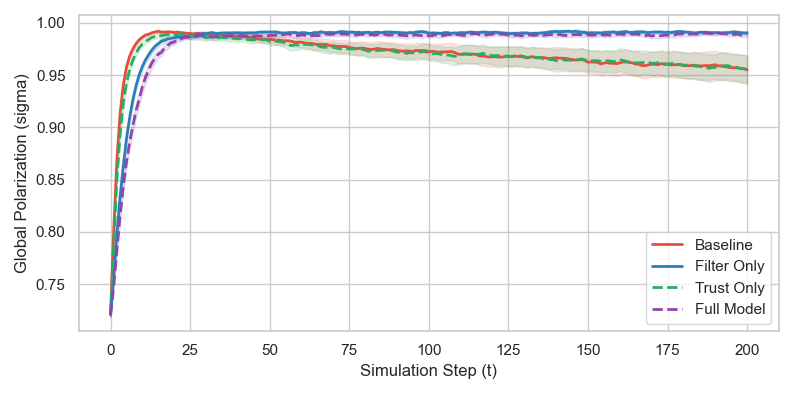
\includegraphics[width=0.58\textwidth]{figures/fig2_polarization_factorial.png}
    \caption{Active-agent polarization ($\sigma$) over time. Filter Only locks survivor polarization higher ($\sigma \approx 0.9904$) than Baseline ($\sigma \approx 0.9550$). This is an active-set / survivorship effect, not a full-population warming (see $\sigma_{\mathrm{all}}$). Error ribbons: $95\%$ CIs.}
    \label{fig:polarization}
\end{figure}

Full-cohort $\sigma_{\mathrm{all}}$ shows no Filter contrast: $0.9904$ vs.\ $0.9905$ ($W = 194.0$, $p_{\text{adjusted}} = 1.000$, $d = -0.004$). Retention effects remain; the claim that the filter \emph{raises} polarization applies to the active-user KPI matching the exit story.

\subsection{Trust Segregation}
Under \textbf{Trust Only}, ingroup trust rises to $0.9808$ ($\text{SD} = 0.0056$, $95\%\ \text{CI} = [0.9788, 0.9827]$) and outgroup trust falls to $0.0432$ ($\text{SD} = 0.0256$, $95\%\ \text{CI} = [0.0348, 0.0528]$; Figure~\ref{fig:trust_seg}). Trust Segregation averages $31.28$ ($\text{SD} = 18.83$, $95\%\ \text{CI} = [24.97, 38.21]$; median $= 26.76$, $\text{IQR} = [17.09, 40.66]$). Versus Baseline: $W = 0.0$, $p_{\text{adjusted}} < 1.2 \times 10^{-7}$ (complete same-direction separation; Baseline segregation is fixed at $1$ when Trust OFF). These contrasts enable trust co-evolution; they are not Filter effects.

\begin{figure}[htbp]
    \centering
    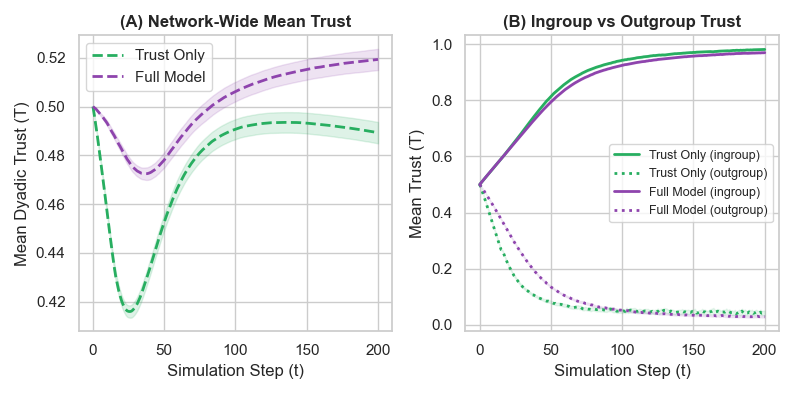
\includegraphics[width=0.65\textwidth]{figures/fig6_trust_dynamics.png}
    \caption{Dyadic trust dynamics. Panel A: mean trust under Trust Only and Full Model. Panel B: ingroup trust (near $0.98$) vs.\ outgroup trust (near $0.04$). Error ribbons: $95\%$ CIs.}
    \label{fig:trust_seg}
\end{figure}

\subsection{Moderation Analysis: Filter \texorpdfstring{$\times$}{x} Trust}
Seed-paired contrasts:
\begin{align}
    \Delta_{\text{alone}} &= \text{Metric}(\text{Filter Only}) - \text{Metric}(\text{Baseline}) \\
    \Delta_{\text{with trust}} &= \text{Metric}(\text{Full Model}) - \text{Metric}(\text{Trust Only})
\end{align}
Wilcoxon tests on $\Delta_{\text{with trust}}-\Delta_{\text{alone}}$ use a separate interaction Bonferroni family of size $m=7$ after excluding trust-KPI rows with $\Delta_{\mathrm{alone}}\equiv 0$ (Table~\ref{tab:interaction}). Those excluded rows are descriptive Full-vs-TrustOnly contrasts on trust metrics, not Filter$\times$Trust moderation. Same-pole triangle purity is included in the family (CSV column \texttt{Opinion\_Clustering}); its interaction is non-significant ($W=168$, adj.\ $p=1$).

\begin{table}[htbp]
\centering
\footnotesize
\caption{Filter $\times$ Trust interaction (seed-paired). Interaction family $m=7$ excludes trust-KPI rows with $\Delta_{\mathrm{alone}}=0$ (shown below the rule for transparency; adj.\ $p$ n/a). Active Users / Churn / Revenue are dependent retention readouts.}
\label{tab:interaction}
\begin{tabular}{lccccc}
\toprule
 & \textbf{Effect Alone} & \textbf{Effect w/Trust} & \textbf{Interaction} & & \\
\textbf{Metric} & \textbf{($\Delta_{\text{alone}}$)} & \textbf{($\Delta_{\text{with trust}}$)} & \textbf{Cohen's $d$} & \textbf{$W$} & \textbf{Adj.\ $p$} \\
\midrule
Active Users & $+194.0$ & $+190.3$ & $-0.3347$ & $117.5$ & $0.1250$ \\
Avg.\ Frustration & $-0.3849$ & $-0.3915$ & $-0.0368$ & $216.0$ & $1.0000$ \\
Churn Rate & $-38.80\%$ & $-38.05\%$ & $+0.3347$ & $121.0$ & $0.1523$ \\
Same-pole purity & $-0.0486$ & $-0.0446$ & $+0.2086$ & $168.0$ & $1.0000$ \\
Polarization ($\sigma$) & $+0.0353$ & $+0.0336$ & $-0.0469$ & $208.0$ & $1.0000$ \\
Polarization ($\sigma_{\mathrm{all}}$) & $+0.0000$ & $-0.0002$ & $-0.0382$ & $221.0$ & $1.0000$ \\
Revenue & $+\$77.60$ & $+\$76.11$ & $-0.3347$ & $111.0$ & $0.0871$ \\
\midrule
Ingroup Trust$^{\dagger}$ & $0.0000$ & $-0.0110$ & $-3.2083$ & $1.0$ & n/a \\
Mean Trust$^{\dagger}$ & $0.0000$ & $+0.0300$ & $+4.9482$ & $0.0$ & n/a \\
Outgroup Trust$^{\dagger}$ & $0.0000$ & $-0.0139$ & $-0.9249$ & $84.0$ & n/a \\
Trust Segregation$^{\dagger}$ & $0.0000$ & $+5.3710$ & $+0.4417$ & $135.0$ & n/a \\
\bottomrule
\multicolumn{6}{l}{\footnotesize $^{\dagger}$ Excluded from Bonferroni $m$: Trust OFF forces $\Delta_{\mathrm{alone}}=0$ (descriptive only).} \\
\end{tabular}%
\end{table}

Retention interactions (Active Users, Churn, Revenue---dependent readouts---and Frustration) remain non-significant after Bonferroni. Some raw $p$-values are $\approx 0.01$--$0.02$ before correction and then fail the $m=7$ family; with $n=30$ we report \emph{no evidence of moderation}, not statistical equivalence of Filter effects with and without trust. Active $\sigma$ likewise shows no Filter$\times$Trust interaction ($W=208$, adj.\ $p=1$).

\subsection{Echo Chambers}
Same-pole triangle purity (local closed active triples; Figure~\ref{fig:clustering}) averages $0.1316$ in Baseline ($\text{SD} = 0.0255$, $95\%\ \text{CI} = [0.1228, 0.1407]$); Trust Only $0.1316$ ($W = 226.0$, $p_{\text{adjusted}} = 1$). Filter Only lowers purity to $0.0830$ ($\text{SD} = 0.0152$, $95\%\ \text{CI} = [0.0776, 0.0884]$, $W = 0.0$, $p_{\text{adjusted}} < 1.2 \times 10^{-7}$, $|d| = 2.32$). Full Model: $0.0870$ ($\text{SD} = 0.0136$, $95\%\ \text{CI} = [0.0821, 0.0919]$, $W = 0.0$, $p_{\text{adjusted}} < 1.2 \times 10^{-7}$, $|d| = 2.19$). The filter can reduce local mono-pole triangles while active-agent $\sigma$ stays high---another active-set / KPI nuance.

\begin{figure}[htbp]
    \centering
    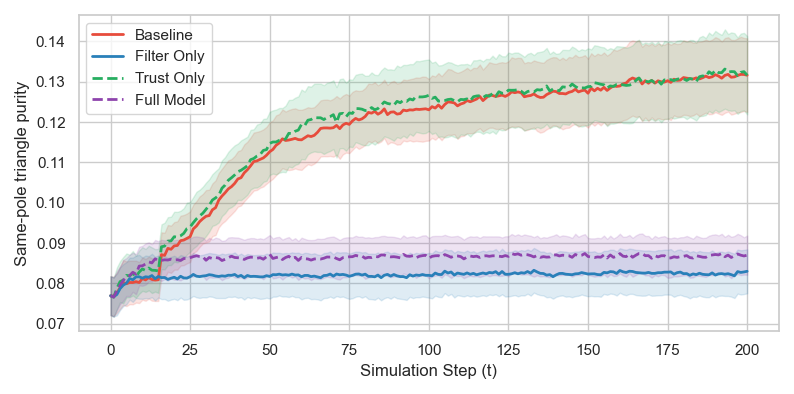
\includegraphics[width=0.58\textwidth]{figures/fig7_echo_chambers.png}
    \caption{Same-pole triangle purity (local closed active triples). Filter ON conditions reduce local mono-pole triangles relative to Baseline while active-agent polarization remains high. Error ribbons: $95\%$ CIs.}
    \label{fig:clustering}
\end{figure}

\subsection{Mechanism Checks}
Descriptive ablations ($20$ seeds; Figure~\ref{fig:ablations}; lower power than the main factorial). Relative to REF (churn $38.66\%$, $\sigma=0.9579$), intercept+heal (M0) yields churn $0.39\%$ and $\sigma=0.9901$. Heal-only (M1) yields churn $5.82\%$. Drop without heal (M2) and intercept with $B_{hb}=0$ (M3) are \emph{identical per seed} under current code (both churn $20.53\%$, $\sigma=0.9839$)---one mechanism identity, not two independent confirmations---and remain distinct from M0. Full Model without trust decay (M4) keeps near-zero churn. Setting the revenue multiplier to $1.0$ (M5) leaves polarization/churn unchanged but scales revenue to the full active-user level.

\begin{figure}[htbp]
    \centering
    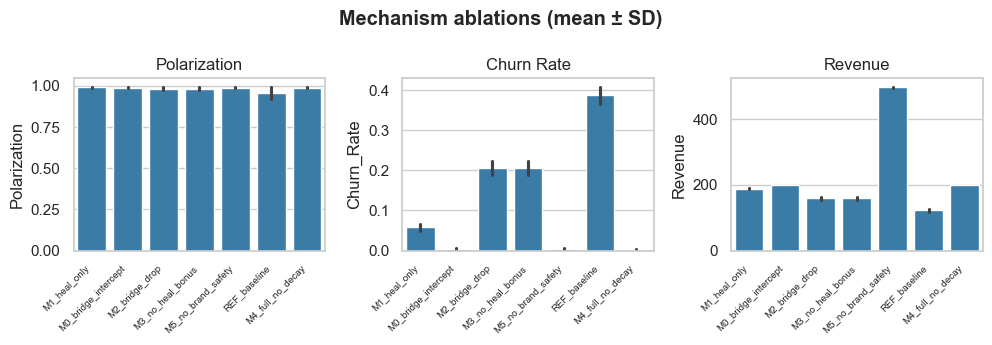
\includegraphics[width=0.95\textwidth]{figures/fig_ablations.png}
    \caption{Mechanism ablations ($20$ seeds): mean Polarization, Churn Rate, and Revenue. Error bars: SDs. Descriptive only.}
    \label{fig:ablations}
\end{figure}

\subsection{Baseline Model Comparison}
On the same BA networks and seeds, HK bounded confidence yields lower final polarization (mean $0.6991$) and no churn pathway. A lightweight biased-assimilation update without SJT zones or exit stays near-extreme (mean $0.9900$) with zero churn. Dynamic-BABE Baseline jointly produces high polarization and substantial exit (Figure~\ref{fig:baselines}).

\begin{figure}[htbp]
    \centering
    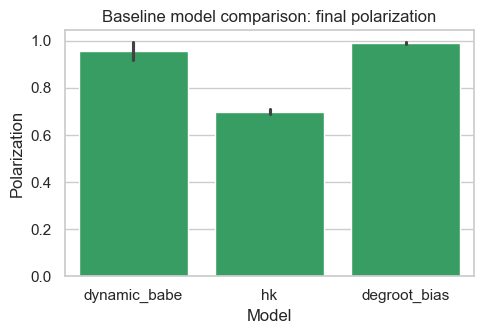
\includegraphics[width=0.55\textwidth]{figures/fig_baselines_polarization.png}
    \caption{Final polarization under Dynamic-BABE Baseline, Hegselmann--Krause, and biased DeGroot-style updates ($20$ seeds).}
    \label{fig:baselines}
\end{figure}

\subsection{Topology Robustness}
Filter OFF/ON on Watts--Strogatz ($k=6$, $p=0.1$; $15$ seeds; descriptive) preserves the qualitative direction: filter cuts churn while active-agent polarization rises, comparable to Barab\'{a}si--Albert under the same seeds (Figure~\ref{fig:topology}).

\begin{figure}[htbp]
    \centering
    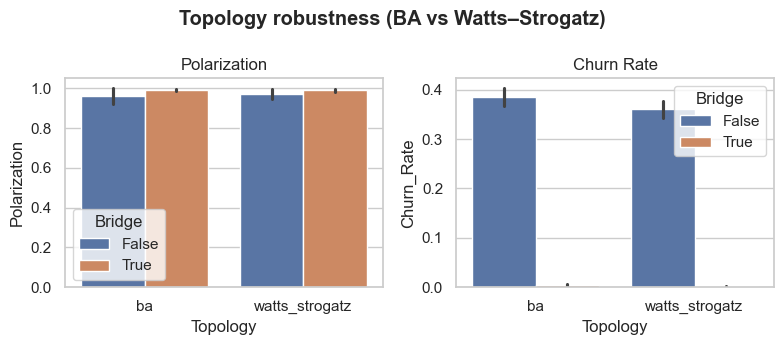
\includegraphics[width=0.85\textwidth]{figures/fig_topology_robustness.png}
    \caption{Filter OFF/ON contrasts on Barab\'{a}si--Albert vs.\ Watts--Strogatz ($15$ seeds). Descriptive.}
    \label{fig:topology}
\end{figure}
